\documentclass[border=5mm]{standalone}
\usepackage{tikz}
\usetikzlibrary{arrows.meta, positioning}

\begin{document}

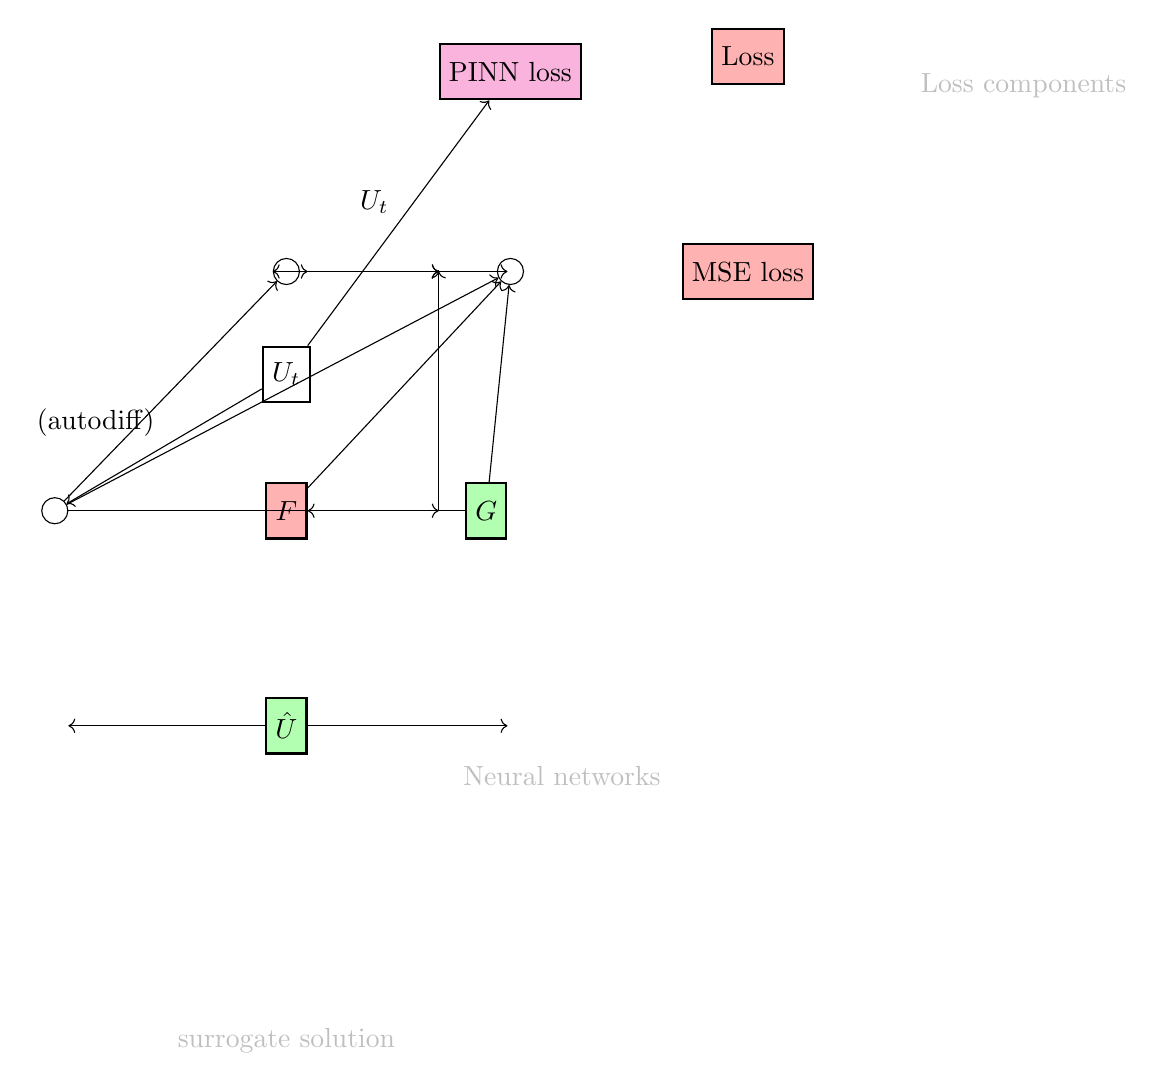
\begin{tikzpicture}[node distance = 2cm,
    block/.style={draw, thick, fill=white!20, minimum height=2em},
    sum/.style={draw, circle, node distance=2.5cm},
    pinstyle/.style={pin edge={to-,thin,black}}
]

% Nodes 
\node [block, fill=red!30] (F) {$F$};
\node [block, right=of F, fill=green!30] (G) {$G$};
\node [block, below=of F, fill=green!30] (U) {$\hat{U}$};
\node [sum, above=of F] (Udot) {};
\node [sum, right=of Udot] (plus) {};
\node [sum, left=of F] (Fdot) {};
\node [block, above=of plus, fill=magenta!30] (PINN) {PINN loss};
\node [block, right=of plus, fill=red!30] (MSE) {MSE loss};
\node [block, above=of MSE, fill=red!30] (Loss) {Loss};
\node [block, above=1cm of F, fill=white!60] (U_t) {$U_t$};

% Connectors
\draw[->] (U_t) -- node[auto] {$U_t$} (PINN);
\draw[->] (U_t) -- node[auto, swap] {(autodiff)} (Fdot);
\draw[->] (Fdot) -- node[auto] {} (Udot);
\draw[->] (Udot) -- (Udot-|PINN.west);
\draw[->] (Fdot) -- (Fdot-|PINN.west);
\draw[->] (Fdot) -- node[auto] {} (plus);
\draw[->] (F) -- node[auto] {} (plus);
\draw[->] (plus) -- (plus-|G.east);
\draw[->] (G) -- node[auto] {} (plus);
\draw[->] (plus) -- (plus-|Udot.west);
\draw[->] (Fdot-|PINN.west) |- (Udot-|PINN.west);
\draw[->] (U) -- (U-|Fdot.east);
\draw[->] (U) -- (U-|G.east);
\draw[->] (G) -- (G-|U.east);
\draw[->] (Udot) -- (Udot-|U.east);
\draw[->] (Udot) -- (Udot-|PINN.west);

% Surrogate Solution
\node at ([yshift=-4cm]U.center) {\textcolor{gray!50}{surrogate solution}};
% Loss Components
\node at ([xshift=3.5cm,yshift=2cm]MSE.north) {\textcolor{gray!50}{Loss components}};
\node at ([xshift=3.5cm,yshift=-1cm]U.north) {\textcolor{gray!50}{Neural networks}};


\end{tikzpicture}

\caption{Overview of the structure of the UPINN method as applied to \eqref{eq:1}. The surrogate solution $\hat{U}$ outputted by the UPINN takes time $t$ as input. Both $F$ (the known component of the differential equation) and $G$ (the unknown component, to be fit by the UPINN) take in time and $\hat{U}$, the prediction of the neural network, as input. $F$ and $G$, along with $U_t$ (the autodifferentiated derivative of $U_{NN}$ w.r.t. time) are passed as input to the PINN loss. Then, the PINN loss computes the error between $U_t$ and $F+G$. The MSE loss computes the error between the surrogate solution $\hat{U}$ and the data.}
\label{fig:UPINN_structure}

\end{document}